Diese Option ähnelte der ersten Option, jedoch mit dem Unterschied, dass die Daten von den Drittsystemen direkt in die Datenbank von Statistance geschrieben werden. Dabei wäre die Datenabholung über einem vorher festgelegten Zeitplan (schedule) in einem Batch-Verfahren oder per API ausgelöst worden, woraufhin die Ergebnisse in die bereits vorhandene relationale Datenbank von Statistance geschrieben worden. Dadurch hätte Statistance die benötigten Daten direkt aus ihrer bereits genutzten Datenbank beziehen können und wäre zudem performanter als die erste Option gewesen. Die benötigten Daten wären vorher durch unsere Applikation in die Datenbank eingespielt worden.
Die Abbildung \ref{fig:Entwicklung einer API & Speicherung in eine Datenbank} stellt die Architektur der Lösung dar.

\begin{figure}[!h]
\centering
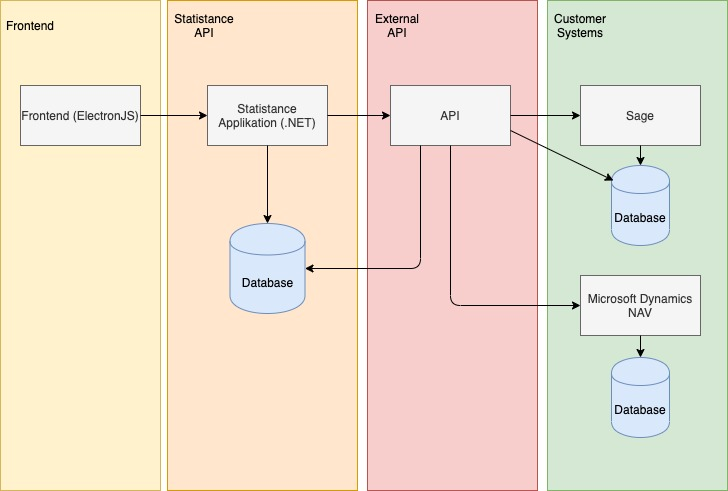
\includegraphics[width=15cm]{images/0x_implementation_possibilities/opt2.jpg}
\caption{Entwicklung einer API \& Speicherung in eine Datenbank}
\label{fig:Entwicklung einer API & Speicherung in eine Datenbank}
\end{figure}

Da wir hierbei auf die bereits genutzte Datenbank von Statistance zurückgegriffen hätten, wären keine weiteren Ressourcen notwendig gewesen und es wäre kein zusätzlicher Aufwand für den Betrieb entstanden. Die Komplexität des Gesamtsystems bliebe dadurch überschaubar und die Kosten blieben weiterhin gering. Allerdings wären durch das Schreiben in die existierende Datenbank auch neue Herausforderungen entstanden. Zum einen wäre das vorhandene Datenbank-Schema von Statistance komplexer geworden, da nun mehr Daten in der gleichen Datenbank gespeichert werden, was zu einem höheren Wartungsaufwand bei der Datenbank führt hätte (insbesondere, wenn die Anzahl der anzubindenden Anwendungen steigt). Zum anderen führte dieser Ansatz zu einer geringen Flexibilität bei Veränderungen in den Anwendungen, da die Anwendungen eng gekoppelt sind und mögliche Abhängigkeiten entstanden wären. Das bedeutet auch, dass Daten in der Datenbank gewesen wären, die Statistance eventuell (noch) nicht benötigt hätte. Allgemein war die Schwachstelle dieser Lösung, dass sie zu unflexibel für künftige Änderungen war, da sie sich zu sehr auf die aktuelle Anwendung inklusive Datenbank von Statistance einschränkt hatte.